% Hur huvudenheten är designad

\section{Huvudenhet}
Huvudenheten har till uppgift att styra roboten. I huvudenheten sitter all systemets intelligens.

\subsection{Hårdvara}
Den hårdvara som ingår i huvudenheten består av en Beagleboard-xm. På denna sitter en Blåtandsdongel monterad för kommunikation med PCenheten. Denna är ansluten till styrenheten och sensorenheten med en flatkabel som innehåller SPI-busen.

\subsection{Mjukvara}
Mjukvaran är uppdelad i fyra trådar. En maintråd som har hand om all styrlogik, en PCtråd som hanterar all kommunikation med PC:n, en sensortråd som kontinuerligt uppdaterar huvudenhetens sensorvärden och en regulatortråd som har hand om regleringen så roboten kan följa banan utan problem. Alla dessa kommunicerar med varandra genom en global datastruktur som innehållar alla olika variabler som behöver delas. Kommandon från PC:n delas mellan pctråden och maintråden genom en kö.

Figur \ref{huvud-tradar} illustrerar dataflödet mellan huvudenhetens olika trådar. Värt att notera är att det finns en tråd dedikerad till vardera extern enhet som kommunicerar med huvudenheten.

\begin{figure}[h!]
	\centering
	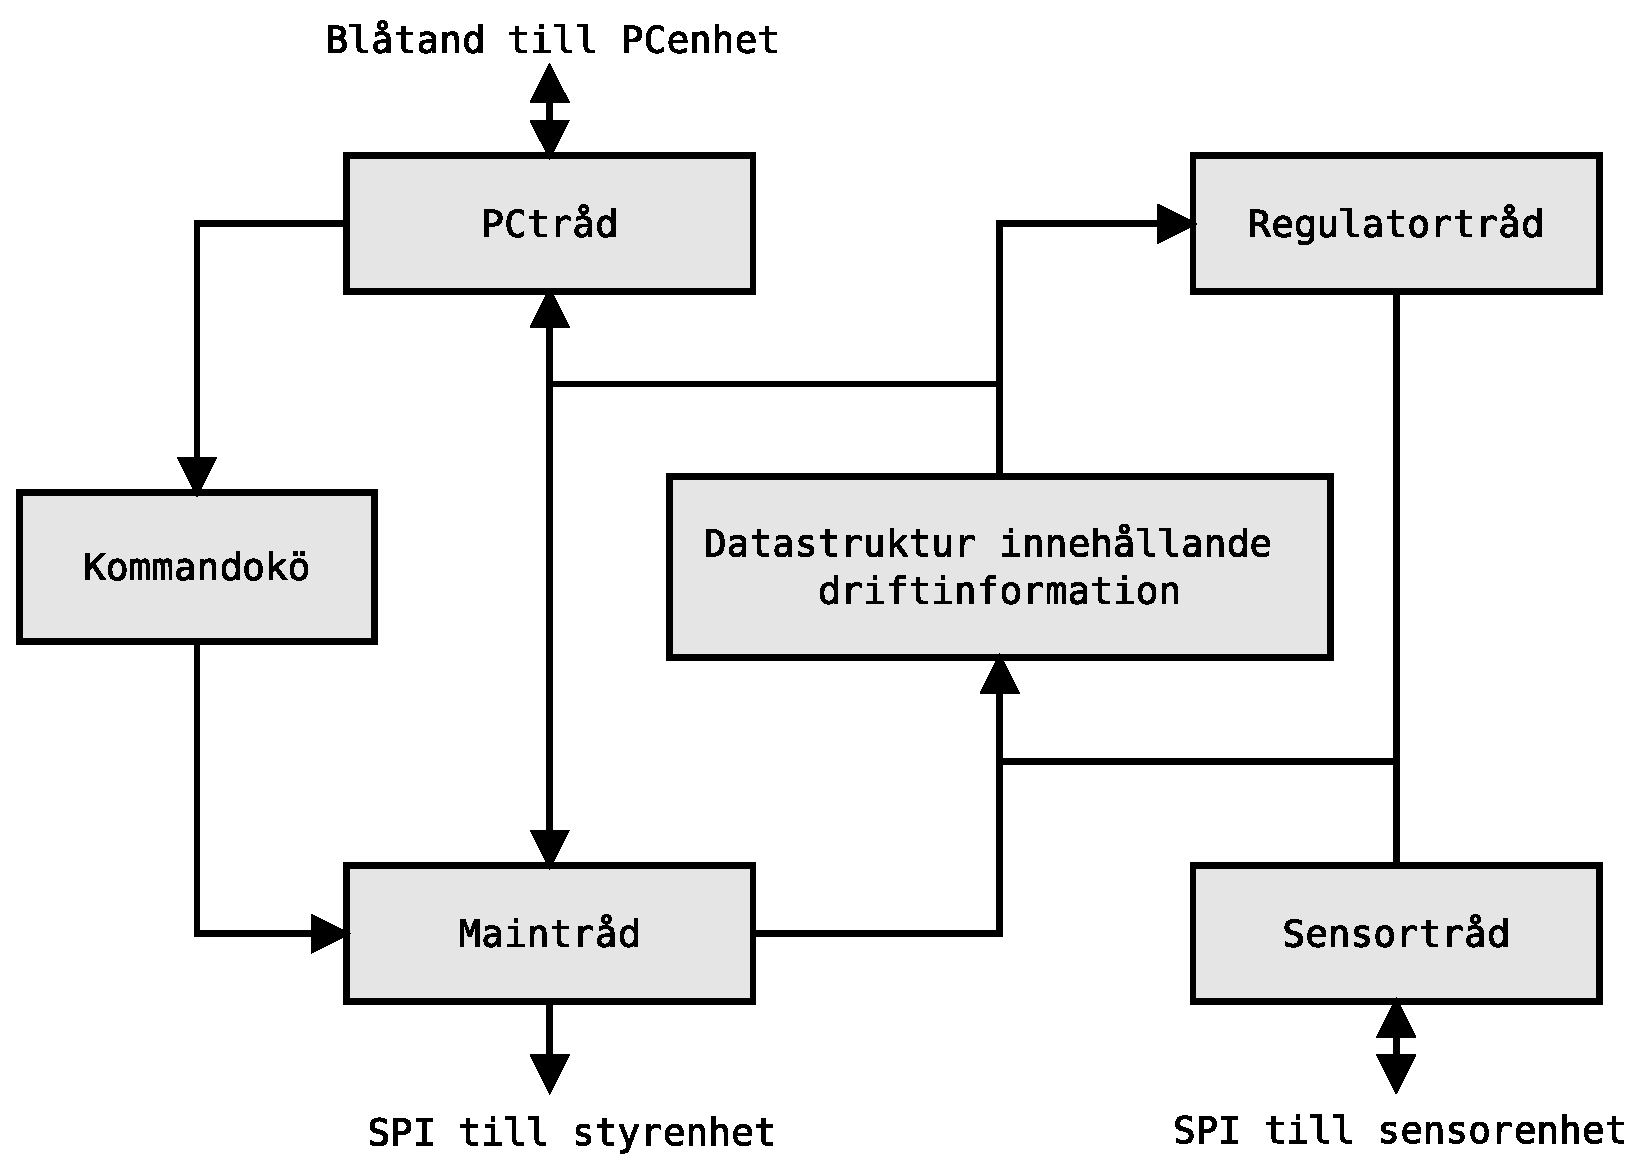
\includegraphics[scale=0.5]{grafik/huvud-tradar}
	\caption{Översikt över huvudenhetens trådar} \label{huvud-tradar}
\end{figure}

\subsubsection{Maintråd}
Maintråden är den tråd som ser till att vår robot faktiskt gör något med den information och de kommandon den tar emot från andra enheter. Tråden avgör vilket tillstånd systemet befinner sig i, om roboten skall köras autonomt beroende på sensordata eller om den bara ska utföra kommandon mottagna från PCenheten.

\paragraph{Tillstånd}

Systemet består av sex olika tillstånd, illustrerade i figur \ref{huvud-tillstand-diagram} och förklarade i tabell \ref{huvud-tillstand}. Det som inte syns i figuren är att systemet kan gå till tillståndet \texttt{MANUAL} även från de tre tillstånden \texttt{STATION FRONT}, \texttt{STATION CENTER} och \texttt{STATION BOTH} och i så fall kommer systemet även återgå till detta tidigare tillstånd från \texttt{MANUAL} då \texttt{autoMotor = True}.

\begin{figure}[h!]
	\centering
	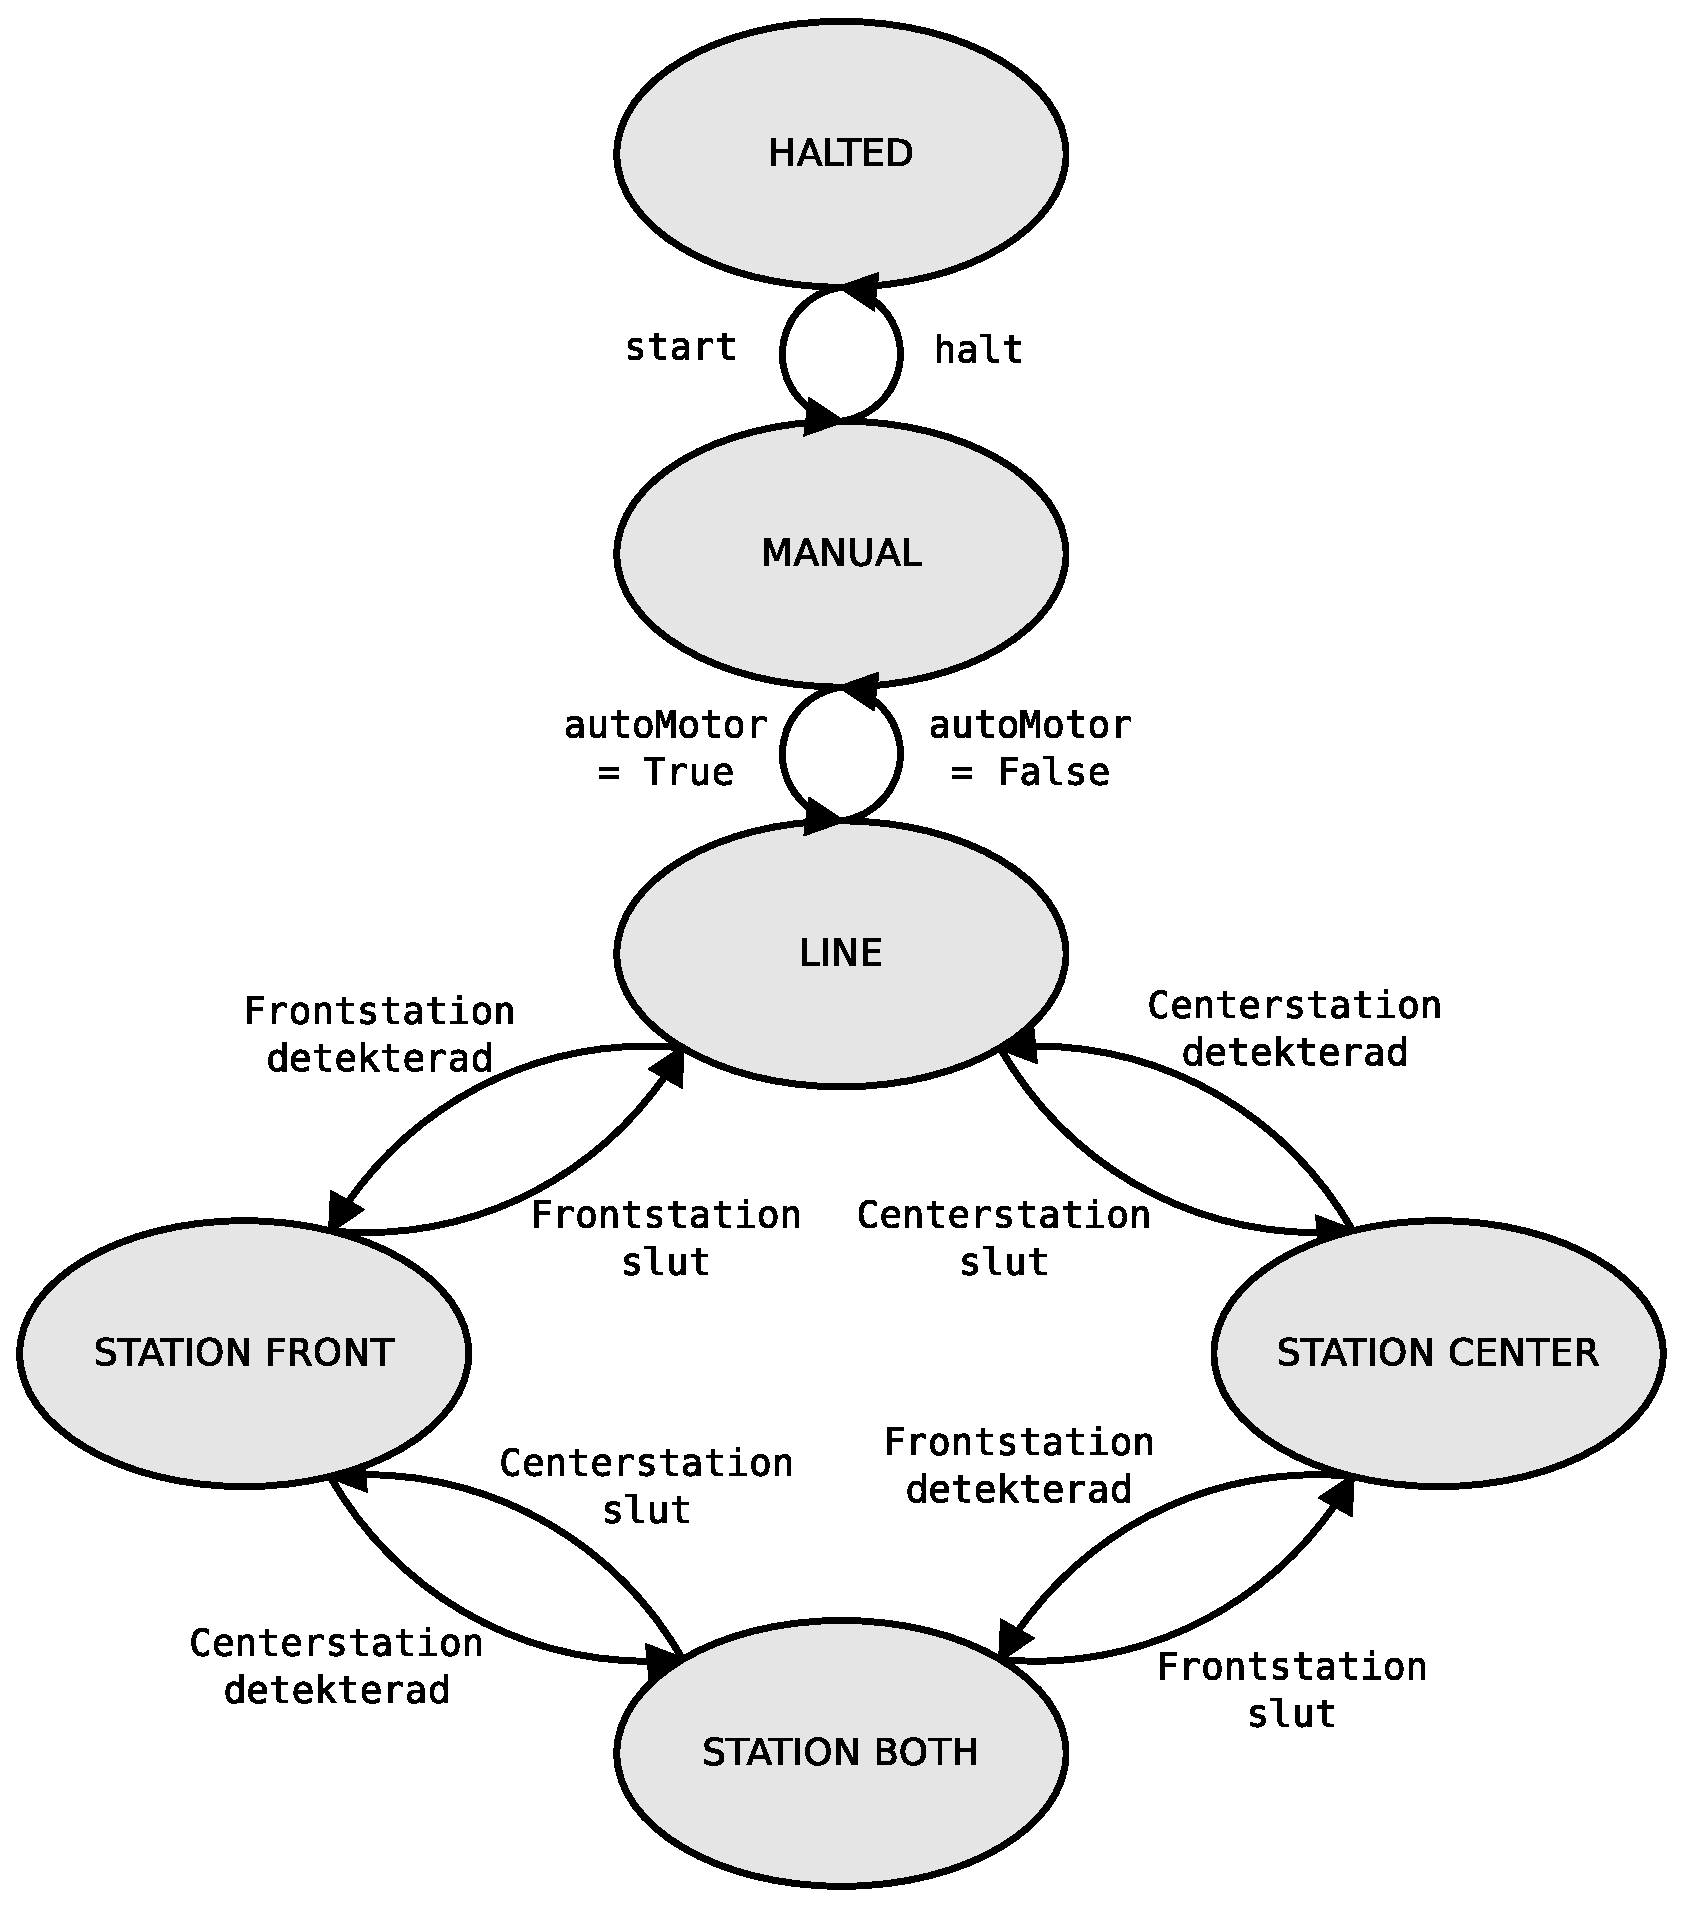
\includegraphics[scale=0.4]{grafik/huvud-tillstand}
	\caption{Översikt över maintrådens olika tillstånd} \label{huvud-tillstand-diagram}
\end{figure}

\begin{table}[h!]
	\centering
	\begin{tabularx}{\textwidth}{| l | X |}
		\hline
		{\textbf{Tillstånd}} & {\textbf{Beskrivning}} \\\hline
		{\texttt{HALTED}} & {Autonom och manuell styrning avstängd.} \\\hline
		{\texttt{MANUAL}} & {Systemet styrs manuellt.} \\\hline
		{\texttt{LINE}} & {Systemet kör autonomt.} \\\hline
		{\texttt{STATION FRONT}} & {Systemet har detekterat en station vid de främre sensorerna.} \\\hline
		{\texttt{STATION CENTER}} & {Systemet har detekterat en station vid de centrerade sensorerna.} \\\hline
		{\texttt{STATION BOTH}} & {Systemet har detekterat stationer vid både de främre och de centrerade sensorerna.} \\\hline
	\end{tabularx}
	\caption{Maintrådens olika tillstånd} \label{huvud-tillstand}
\end{table}

\paragraph{Detektion av stationer}

Det finns många potentiella felkällor vid detektion av stationer. Vi skulle kunna få en störning på utsignalen från våra analoga sensorer, underlaget kanske inte är helt homogent och regleringen skulle kunna få oss att momentant stå snett i en korsning. För att motverka dessa felkällor har vi olika typer av filter.

Vi filtrerar spikar från avståndssensorerna genom att vi lagrar de 10 senaste uppmätta värdena, viktar dessa med en binär skala ($D_{n}*2^{-n}$, där $D$ är uppmätta värden och $n$ är index i listan där $0$ är det senaste och $10$ det äldsta uppmätta värdet) och resultatet säger vi är det uppmätta avståndet.

Det finns inte samma möjlighet att filtrera utdata från linjesensorerna på samma sätt, då vi även kan få fel på grund av reglering eller att en tejp i banan inte är helt rak. För varje iteration av sensordata från linjesensorn har vi en rad om 11 data. Istället för att filtrera vardera av dessa 11 data för sig, accepterar vi att ett fåtal av dessa data är avvikande. Den främre linjesensorn delas upp i segment enligt figur \ref{huvud-linjesensor} och för varje segment sätts ett krav för när detta segment kan betraktas detektera en faktisk tejp. För \textit{Höger} och \textit{Vänster} är kravet att tre av fyra sensorer är över tröskelvärdet. För \textit{Mitt} är kravet endast att en sensor är över tröskelvärdet. Endast två av sensorerna på den centrerade linjesensorn används, den har alltså endast två segment bestående av en sensor var, \textit{Center-höger} och \textit{Center-vänster}.

\begin{figure}[h!]
	\centering
	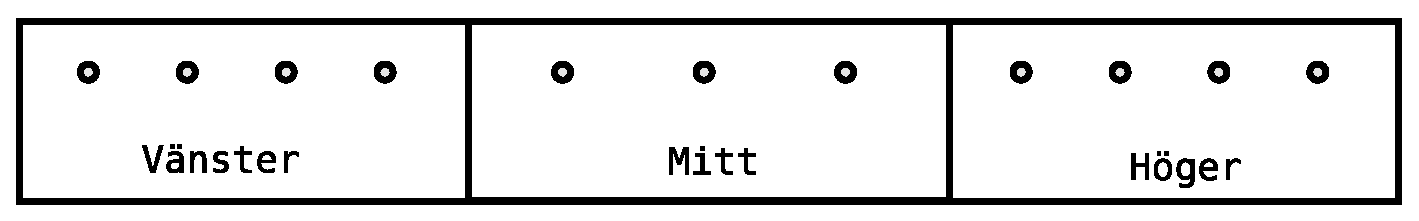
\includegraphics[scale=0.4]{grafik/huvud-linjesensor}
	\caption{Linjesensorn är uppdelad i segment} \label{huvud-linjesensor}
\end{figure}

För att inte upptäcka samma station flera gånger på grund av reglering eller sned bana och för att inte upptäcka en station i en korsning finns det även en mekanisk till. Varje iteration av sensordata sparas i en lista med de senaste sex iterationerna av sensorvärden. När vi sedan ska undersöka om det verkligen är en station vi är vid, går vi igenom alla sex iterationer av sensordata. Om minst fyra av dessa rader av sensordata uppfyller kraven för en station, korsning eller ett avbrott i banan säger vi att så är fallet.

En station kännetecknas av att den ena av \textit{Höger} och \textit{Vänster} detekterar en tejp samtidigt som den inte gör det och vi också har tejp i \textit{Mitt}-segmentet. Skulle alla segment detektera en tejp har vi en korsande väg i banan som skall ignoreras och skulle inget segment detektera tejp har vi ett avbrott i banan.

Vi gör på motsvarande sätt för att detektera att en station är rakt under roboten. Där kräver vi att minst en sensor på \textit{Mitt}-segmentet på frontsensorn ska vara över tröskelvärdet i minst fyra av sex iterationer för att försäkra oss om att vi är på en någorlunda rak linje. Vidare kräver vi att de centrerade sensorerna ska vara över tröskelvärdet i minst fyra av de sex lagrade iterationerna.

\subsubsection{PCtråd}
PCtråden sätter upp en socket när den skapas och väntar på en inkommande anslutning från en PC. När den får en anslutning så väntar den på ett kommando.

Oftast tas flera kommandon emot samtidigt och PCtråden gör om dessa till en lista av kommandon som den går igenom och behandlar ett efter ett. Får man till exempel in två kommandon om sätta motorhastigheten så ser tillvägagångssättet ut på följande sätt:
\begin{enumerate}
\item ";motorSpeed=speed1,speed2;motorspeed=speed3;speed4;" tas emot
\item detta görs om till [["motorspeed",["speed1","speed2"]],["motorSpeed",["speed3","speed4"]]]
\item det första kommandot behandlas genom att argumenten omvandlas till heltal, motorernas hastighet uppdateras i dictionaryt och kommandot läggs till i kön så maintråden vet att den ska skicka ut kommandot.
\item nästa kommando behandlas på samma sätt men om speed1=speed3 och speed2=speed4 så ignoreras kommandot då det inte påverkar hastigheterna.
\end{enumerate}

\subsubsection{Sensortråd}
Sensortråden hämtar data från Sensorenheten med en given uppdateringsfrekvens. De hämtade sensorvärdena normaliseras och lagras i den globala datastrukturen. Normaliseringen utförs på så sätt att sensordatan jämförs med de värden vi fått genom kalibrering, som i ekvation \ref{huvud-eq1}. Den normaliserade sensordatan är alltså hur stor del av det använda intervallet som används.

\begin{equation} \label{huvud-eq1}
	D_{norm}=\frac{D_{in}-D_{min}}{D_{max}-D_{min}}
\end{equation}

\subsubsection{Regulatortråd}
Regulatortråden använder data från linjesensorerna för att beräkna hur roboten behöver röra sig för att följa linjen. Detta görs sedan om till motsvarande motorhastigheter och lagras i den globala datastrukturen.

Regleringen utförs i en egen tråd för att säkerhetsställa att beräkningarna sker med jämna tidsintervall. Det är dock värt att notera att detta tidsintervall är beroende av det tidsintervall med vilket sensortråden uppdaterar sensordata eftersom det är meningslöst att reglera på gamla sensorvärden.
